\documentclass[capstone_report.tex]{subfiles}
\begin{document}
\chapter{Testing and results}
This chapter provides a systematic presentation of test cases and results. Our testing driven development methodology is present first, followed by mapping test cases and finally flight and navigation tests. 

\section{Testing methodology}
During testing, the project team relied heavily on the simulation environment. Code was only tested on a live UAV after it had been vetted by multiple team members in a simulation environment. This allowed us to reduce the chance of a catastrophic collision during a live flight.\\

Despite this, we did still encounter some edge cases which almost caused collisions. For example, we found that in a live environment it took a number of seconds for the EKF position lock to become available. Attempting to takeoff before this time would lead to the drone attempting to fly into the ceiling. Fortunately in this case and many others, we caught this bug before the risk materialised. However, in future it may be advisable to have a more rigourous process in place for real-life indoor UAV testing.\\

Real life testing was predominantly undertaken in the Terabit Networking Lab in the University’s Electrical Engineering faculty building, with chairs and people acting as obstructions and corners. A waypoint was set, the drone was held onto (to prevent accidental collisions) and the results were observed by the team.\\

A large number of tests and edge cases were encountered, so the tests were not formalised in each case. However, a wide range of room configurations were set up and tested in to ensure that the scope objectives and behaviours listed above were met. Improper behaviour, such as overshoot and the following of non-optimal trajectories were removed through continual amending of algorithms.

\section{Mapping tests and results}

One of the primary objectives of this project was to produce an accurate 2D map in real-time.  To test this capability, we deployed the drone in a small room which had previously been measured by a tape measure. The test was undertaken in the same room at two different heights: \SI{40}{\centi\metre} and \SI{80}{\centi\metre}. The room was intentionally configured to have certain measurable obstacles.\\

Figure \ref{fig:map_env_imgs} shows photographs of the test environment at 80cm and 40cm respectively. In each case, URSA was instructed to rotate and move around the room until a measurable map was generated. URSA was then instructed to land and the map generated by URSA was compared to the previous tape measurements collected.\\

\begin{figure}[H]
    \centering
    \begin{subfigure}{0.5\textwidth}
        \centering
        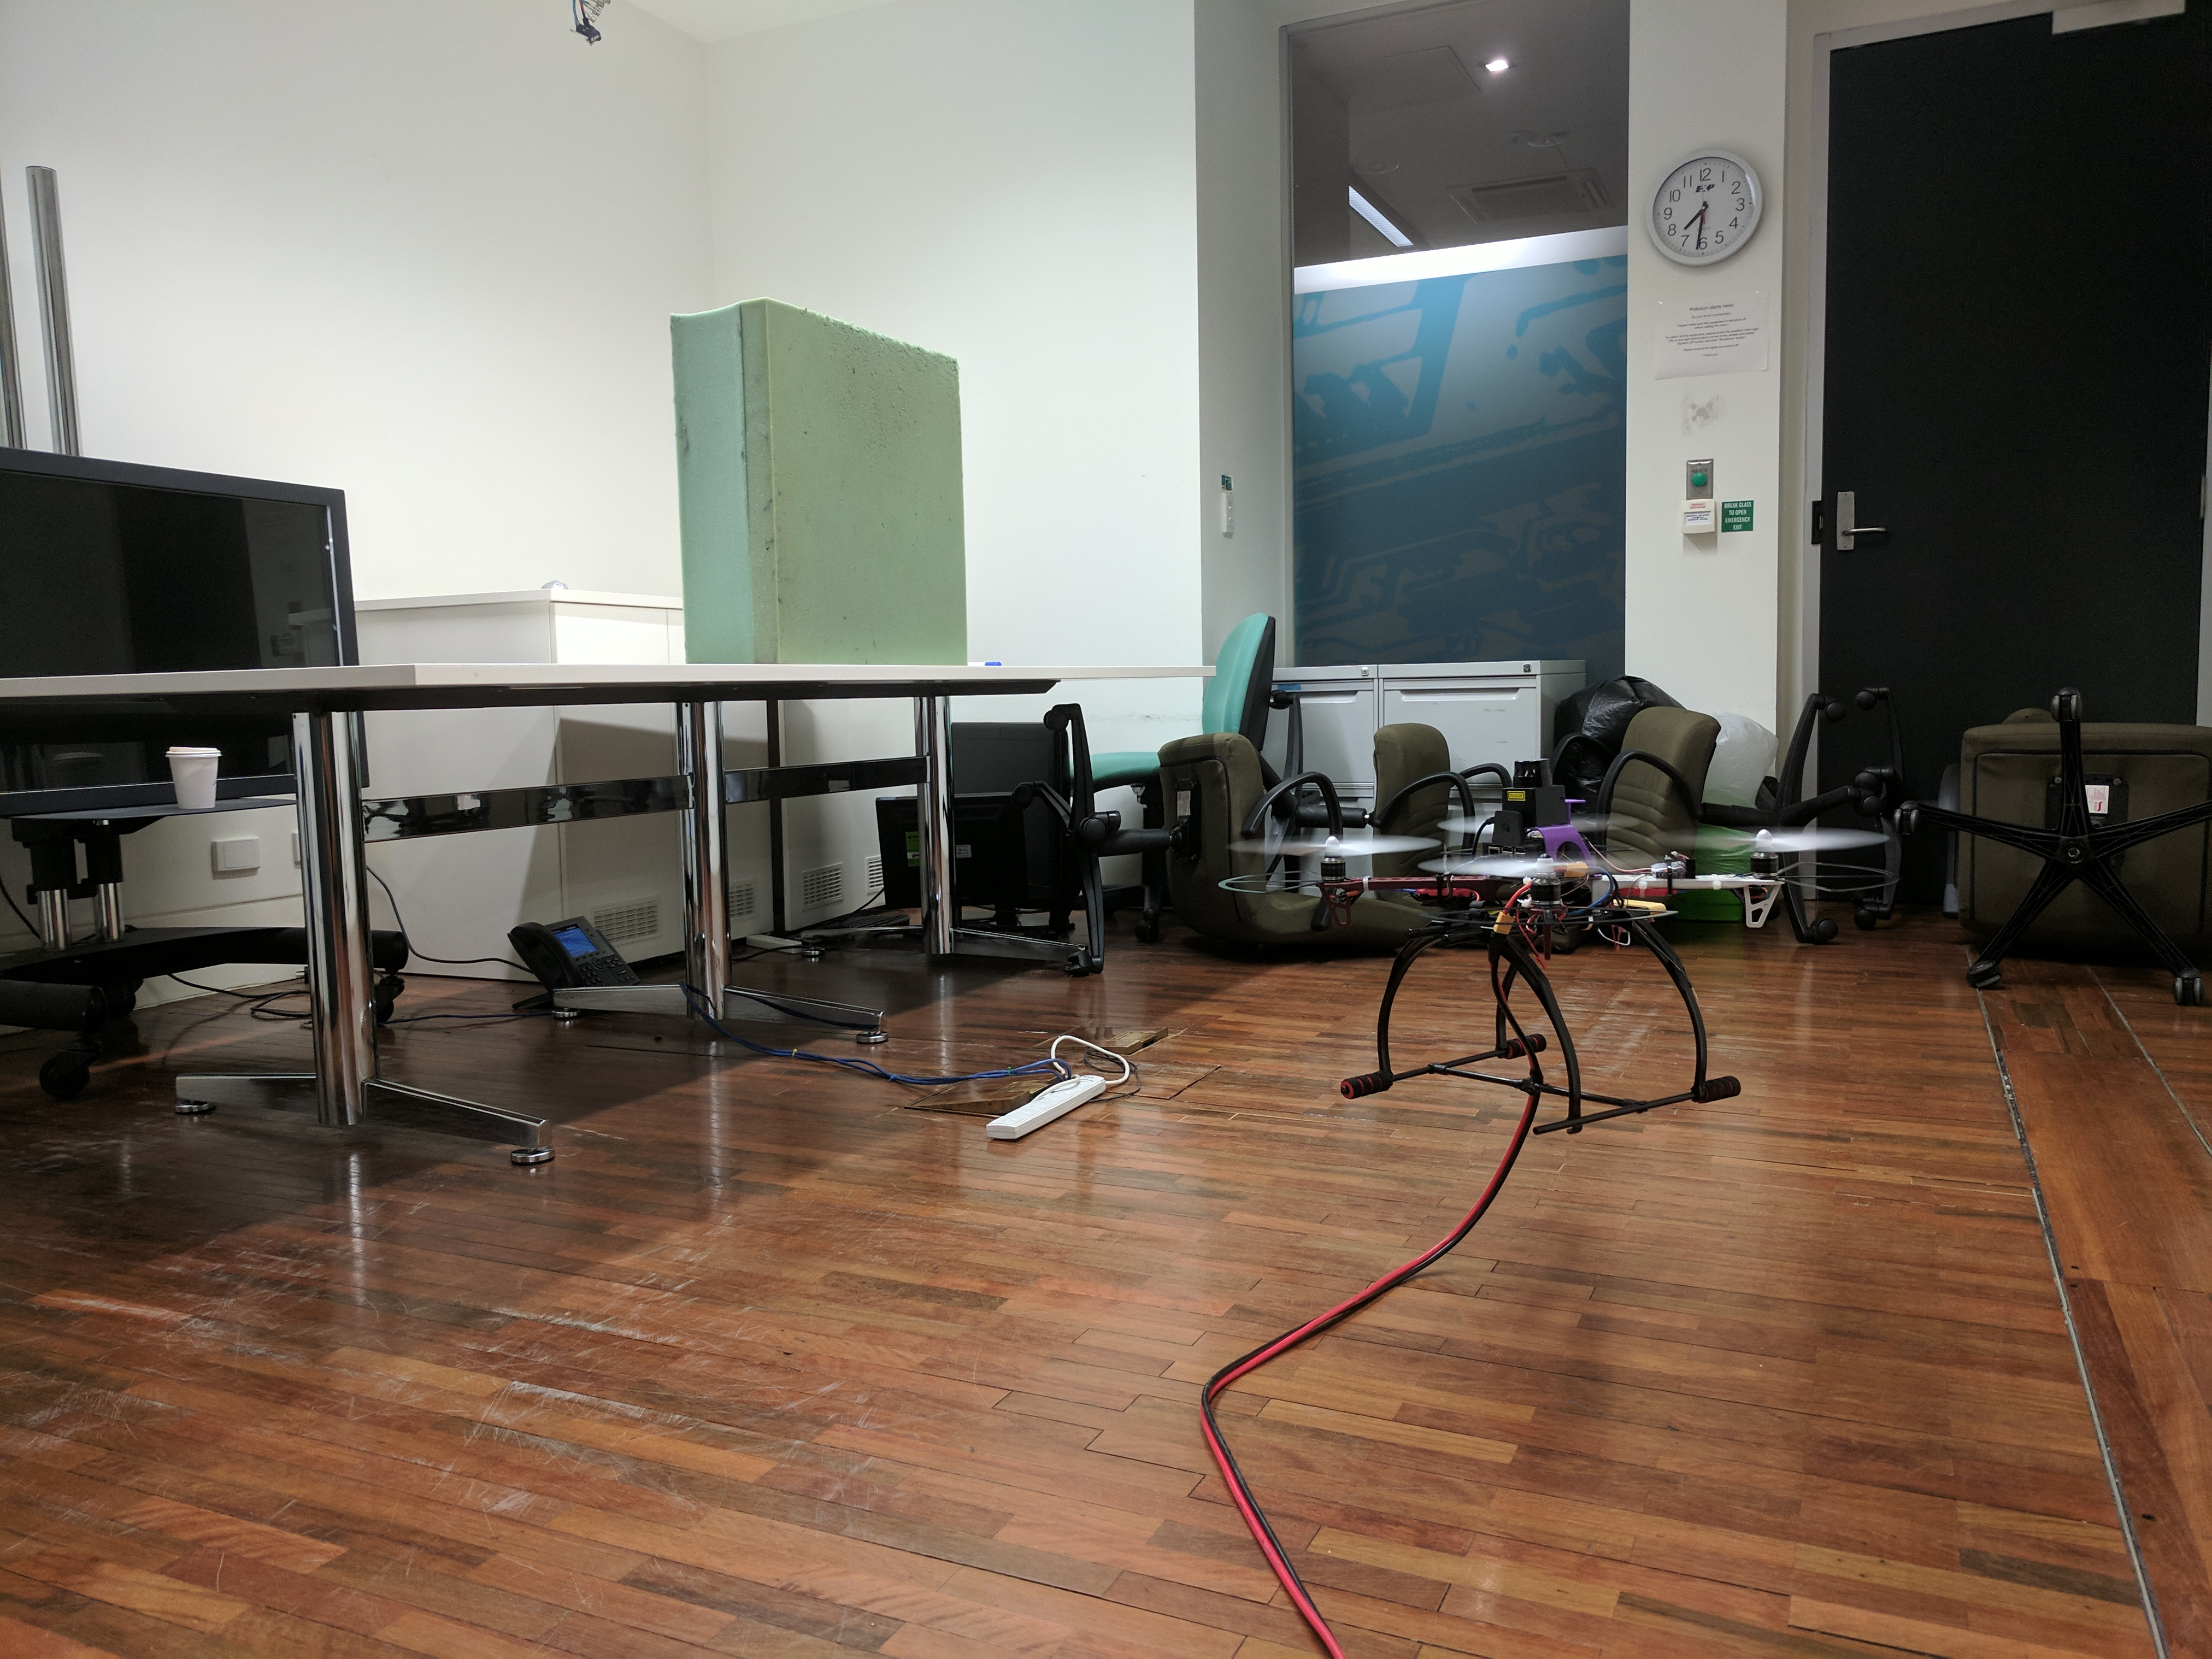
\includegraphics[width=0.9\textwidth]{./imgs/mapping/img_40cm.jpg}
        \caption{40cm}
    \end{subfigure}%
    \begin{subfigure}{0.5\textwidth}
        \centering
        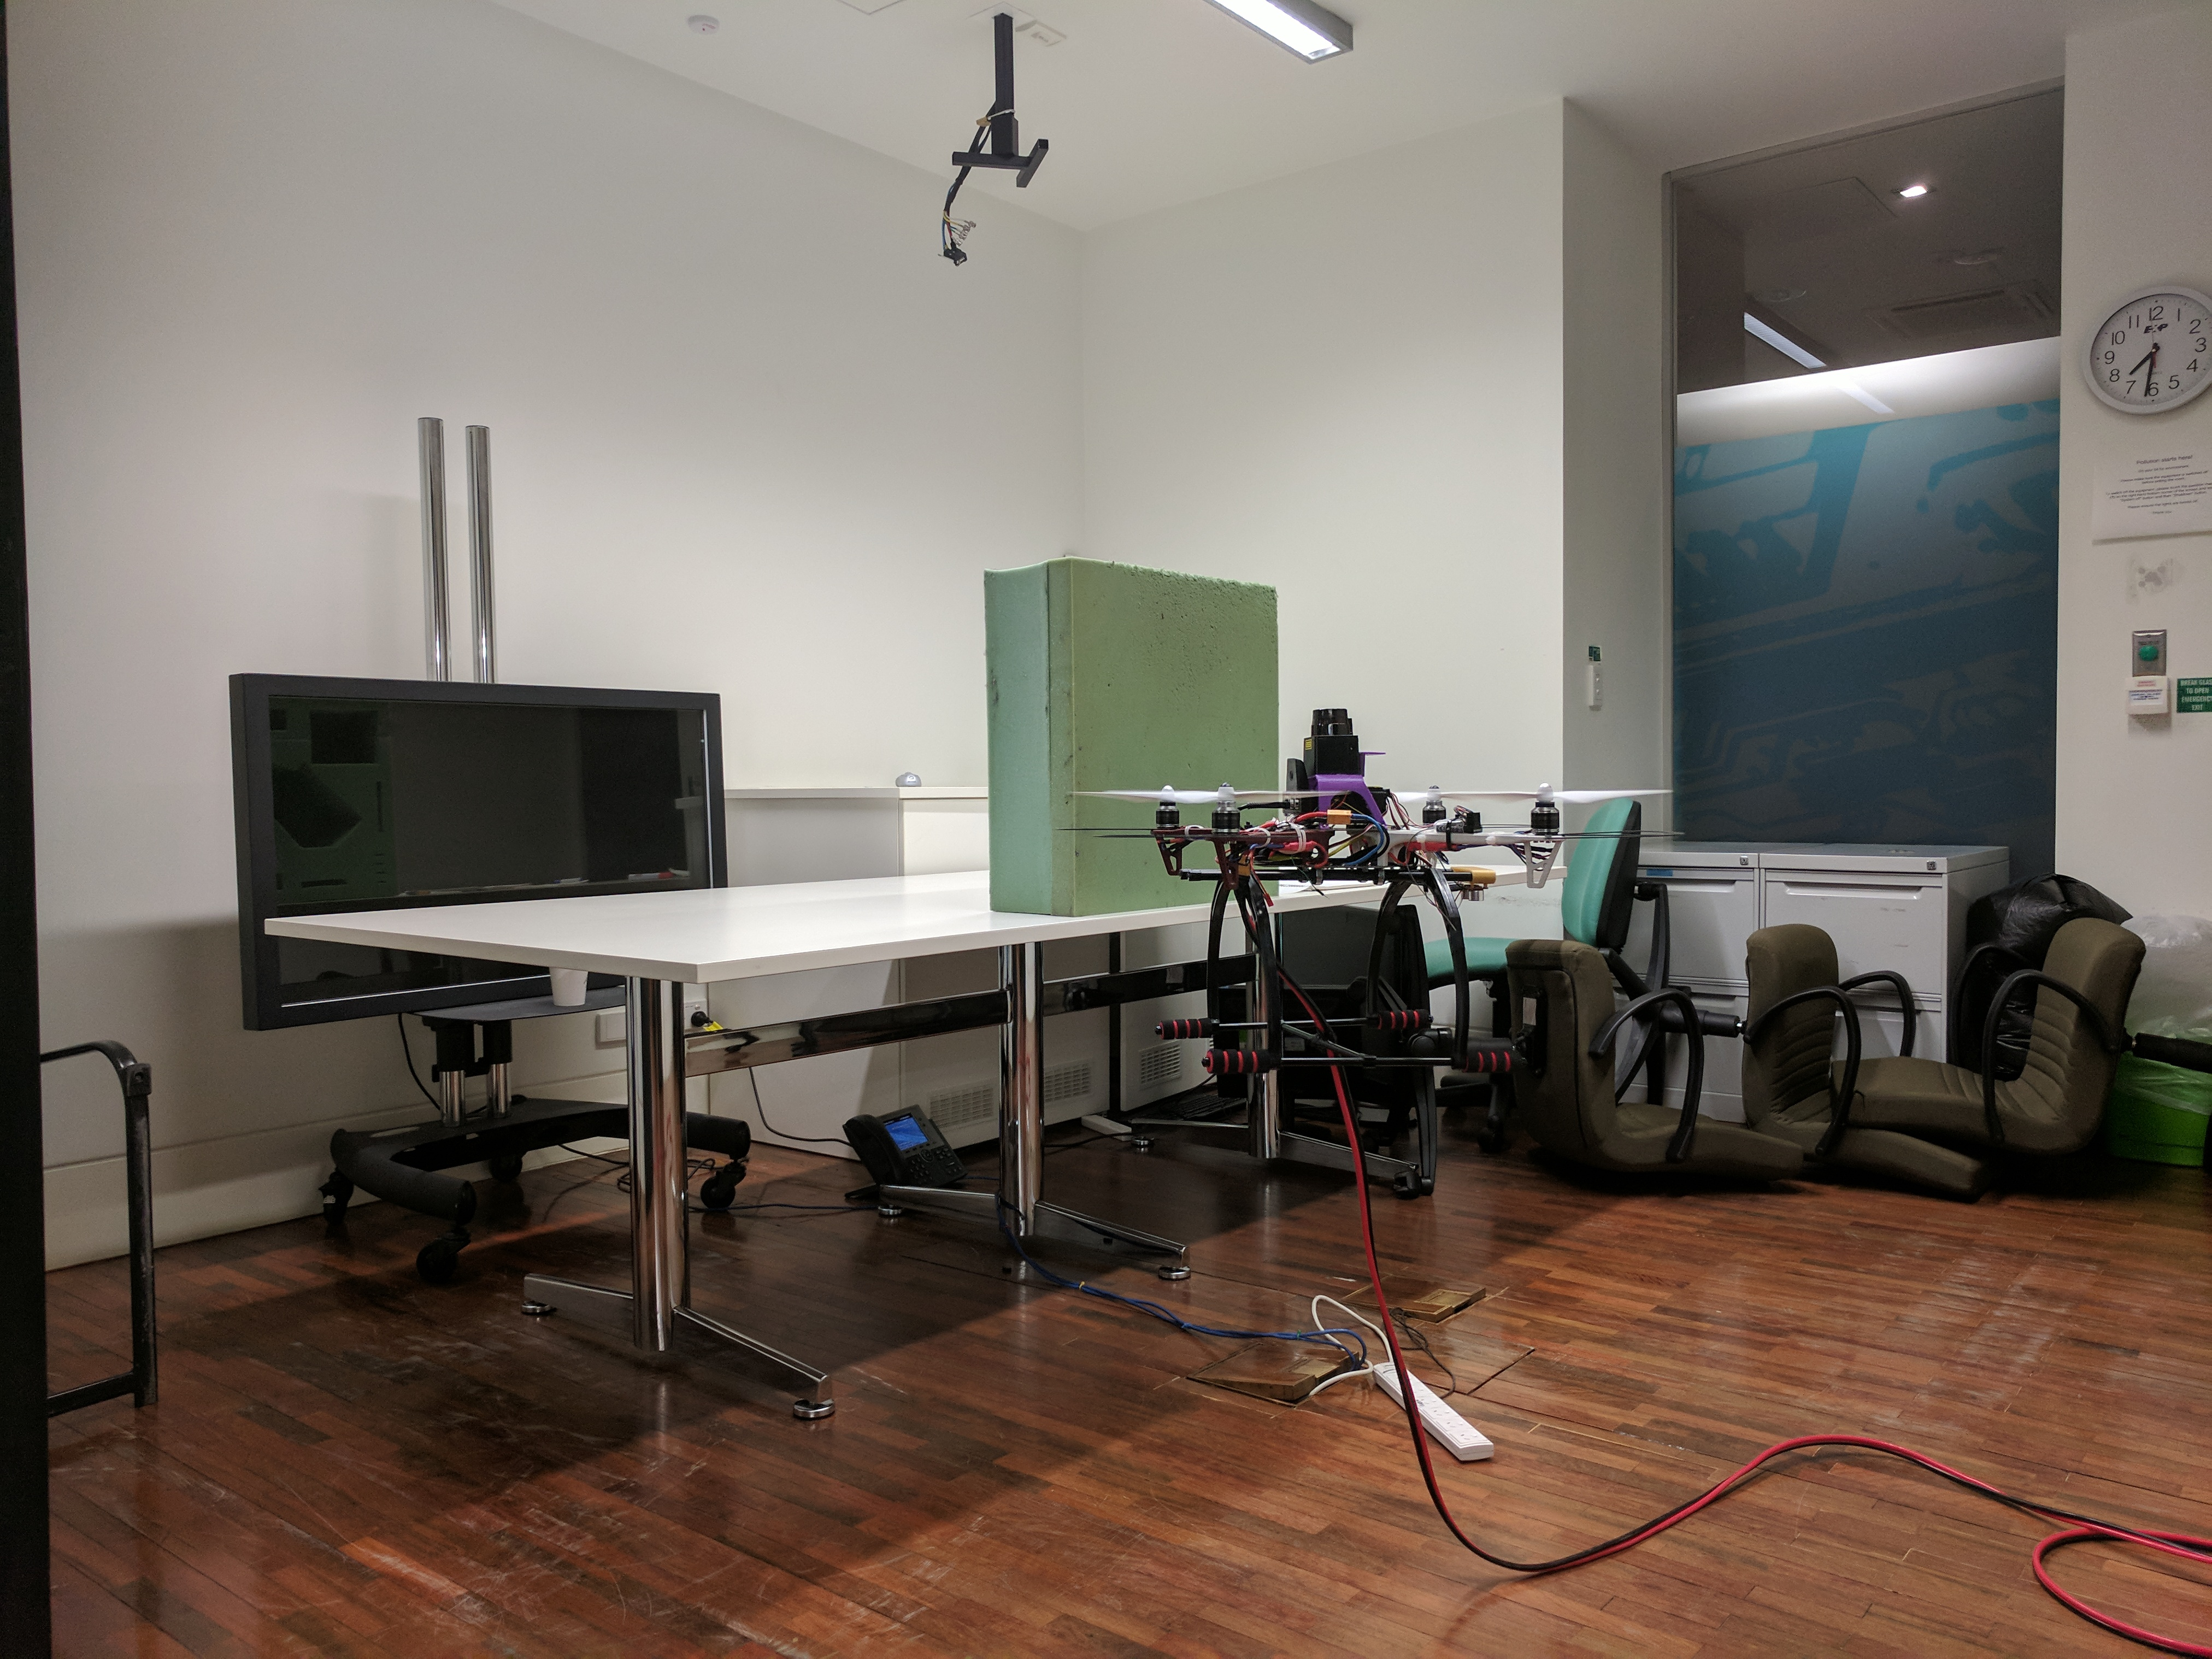
\includegraphics[width=0.9\textwidth]{./imgs/mapping/img_80cm.jpg}
        \caption{80cm}
    \end{subfigure}
    \caption{Photos of experimental setup at multiple flight altitudes}
    \label{fig:map_env_imgs}
\end{figure}

Figure \ref{fig:map_env_RVIZ} shows the 2D map output constructed from sequential laser scans at each 40cm and 80cm. Table \ref{table:measure} summarises the measurements obtained.

\begin{figure}[H]
    \centering
    \begin{subfigure}{0.5\textwidth}
        \centering
        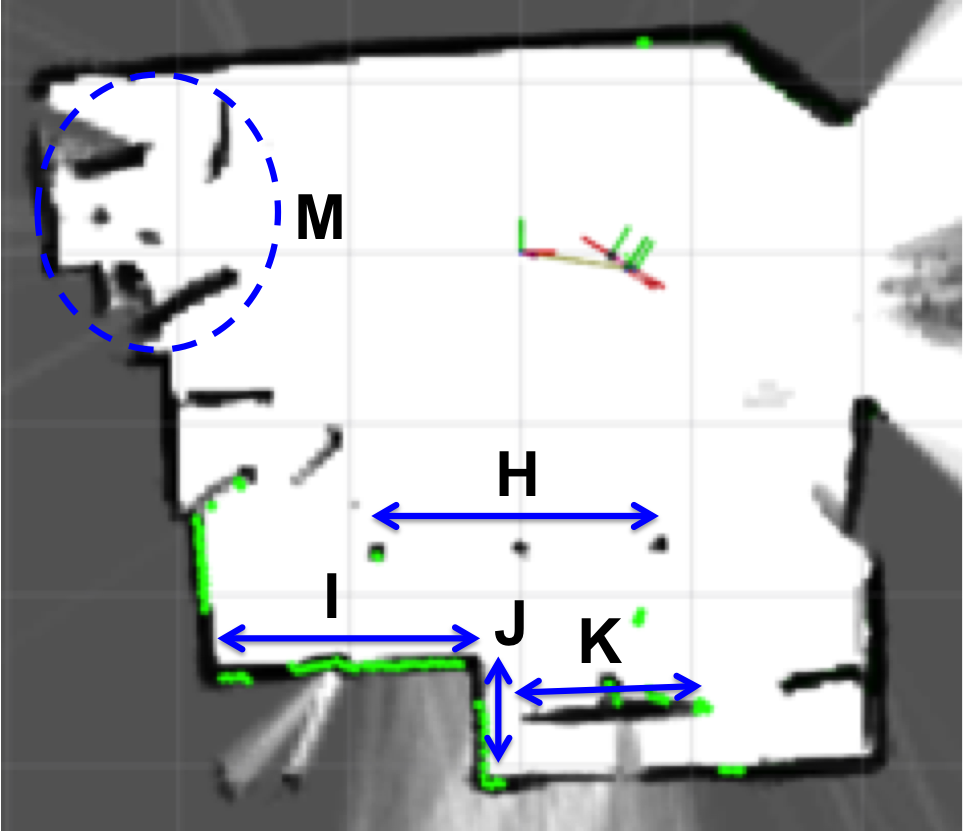
\includegraphics[width=0.9\textwidth]{./imgs/mapping/an_map_40cm_arrows.png}
        \caption{40cm}
    \end{subfigure}%
    \begin{subfigure}{0.5\textwidth}
        \centering
        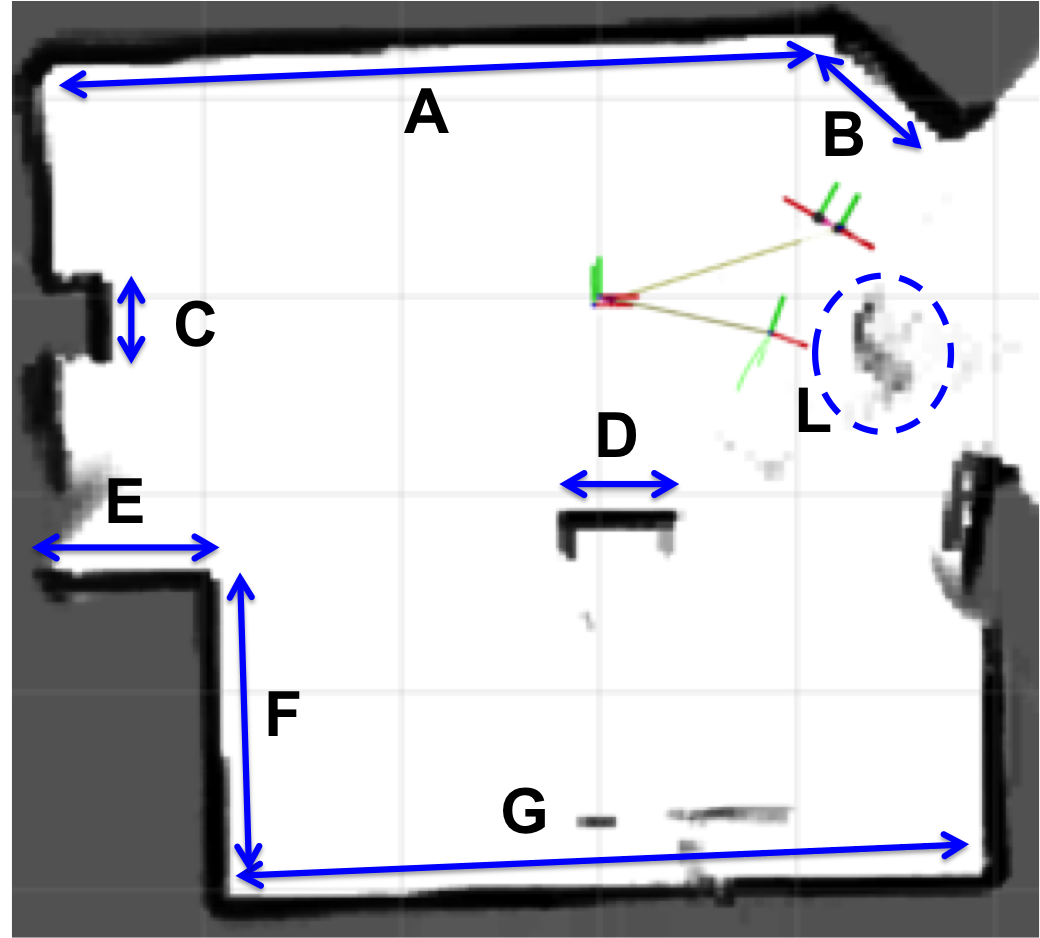
\includegraphics[width=0.9\textwidth]{./imgs/mapping/an_map_80cm_arrows.png}
        \caption{80cm}
    \end{subfigure}
    \caption{Measurements obtained using SLAM algorithm output}
    \label{fig:map_env_RVIZ}
\end{figure}

The results show that there is only a $2cm$ discrepancy between those measurements obtained by hand and those by laser.  The accuracy of a tape measure is with $\pm \frac{1}{2}$ the smallest measurement unit (1cm), therefore this can partly explain for the difference in measurements.  However, as the intended use of the map is high-level strategic planning a $2cm$ accuracy meets the project objective. \\

\begin{table}[H]
\centering
\begin{tabular}{@{}|ccc|@{}}
\toprule
&Tape Measure (m) & Mapping (m)       \\ \midrule
A            & 4.65    & 4.67 \\
B            & 0.82    & 0.81 \\
C            & 0.4     & 0.39 \\
D            & 0.56    & 0.54 \\
E            & 0.75    & 0.75 \\
F            & 1.68    & 1.67 \\
G            & 3.9     & 3.94 \\
H            & 1.7     & 1.69 \\
I            & 1.57    & 1.53 \\
J            & 0.73    & 0.75 \\
K            & 1.12    & 1.06 \\ \bottomrule
\end{tabular}
\caption{Measurements of room obtained by tape measure and laser scans}
\label{table:measure}
\end{table}

Further analysis of the results shows some clear features which can be observed by comparing the maps at 80cm and 40cm. For example, in the map at 80cm the large foam block is clearly visible in the map (marked D in Figure \ref{fig:map_env_RVIZ}). In contrast, on the 40cm map the legs of the table generate three distinct `dots' on the map at around the same location (marked H in Figure \ref{fig:map_env_RVIZ}).\\

Furthermore, in \ref{fig:map_env_RVIZ} there is clearly a discrepancy between the measurement marked G at 80cm and the measurements around I and J at 40cm. This is due to a cupboard which is in the corner of the room, observable at 40cm but not 80cm.\\

Two additional features of Figure \ref{fig:map_env_RVIZ} are worth identifying. The first, marked L in the 80cm results, show a blurry patch which might represent an object. This is actually the result of the drone testers moving near the drone during the test. Since they are not always detected (we moved in and out of the room during the test) the SLAM algorithm is unsure whether this space is actually occupied.\\

The second feature is marked M in Figure \ref{fig:map_env_RVIZ}. This patch of obstacles corresponds to chairs which have been turned over (visible in Figure \ref{fig:map_env_imgs}). These obstacles are observable at 40cm but not 80cm.\\

The analysis also reveals some significant limitations of the mapping scheme chosen. As can be seen in Figure \ref{fig:map_env_imgs}, at both 80cm and 40cm URSA can clearly not navigate over or under the table in the room. Despite this, the table does not feature in either map. This is a significant limitation caused by using 2D mapping rather than 3D mapping.\\

Additionally, in Figure \ref{fig:map_env_RVIZ} near label E, a blurry region of uncertainty can clearly be identified. This is associated with a glass window pane which can be observed in Figure \ref{fig:map_env_imgs}. The laser scanner is not able to detect translucent objects, another significant limitation.

\section{Flight navigation tests and results}
In addition to mapping, it is important that URSA be able to properly navigate complex environments. Tests were undertaken to show that URSA was capable of some fundamental navigation behaviours: avoiding collisions, avoiding obstacles with sufficient clearance, properly orienting itself before moving forwards, and lastly, reach its set destination.\\

Videos for each of the experiments conducted below can be found in the appendix.

\subsection{Avoiding Dynamic Obstacles}
To test URSA's capability to avoid moving obstacles the following experiment was conducted:
\begin{enumerate}
    \item The drone was sent a goal setpoint from its current position
    \item The path from the current drone position to the goal setpoint was unobstructed
    \item As the drone was navigating along the path an obstacle (human) would obstruct its path
\end{enumerate}
Success was measured if the drone was able to generate a trajectory around the obstacle, avoid a collision and reach the original goal setpoint.  The location of the dynamic obstacle was chosen such that a path still existed between the drone and the goal within reasonable margins of obstacles.  Figure \ref{fig:avoid_obs} shows the real-time output to RVIZ when the experiment was conducted in the Terabit Networking Lab (TNL).

\begin{figure}[H]
    \centering
    \begin{subfigure}[b]{0.5\textwidth}
        \centering
        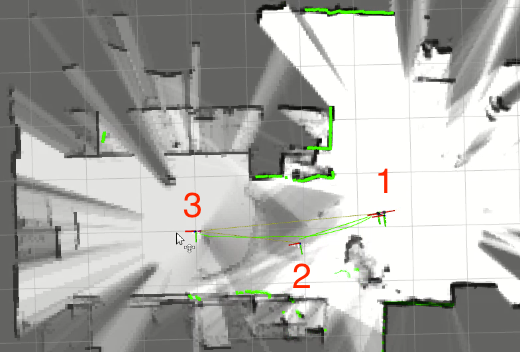
\includegraphics[width=0.97\textwidth]{./imgs/dynamic_objects/an_frame_1.png}
        \caption{Frame 1: Generated trajectory to goal}
        \label{fig:avoid_obs_1}
    \end{subfigure}%
    \begin{subfigure}[b]{0.5\textwidth}
        \centering
        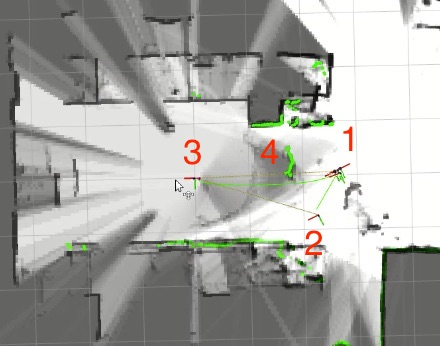
\includegraphics[width=0.97\textwidth]{./imgs/dynamic_objects/an_frame_2.png}
        \caption{Frame 2: Re-generated trajectory}
        \label{fig:avoid_obs_2}
    \end{subfigure}
    \caption{Experiment conducted showing drone avoiding dynamic obstacles.  (1) Drone location (2) Local trajectory goal (3) Global goal (4) Dynamic obstacle\label{fig:avoid_obs}}
\end{figure}

Figure \ref{fig:avoid_obs_1} shows the first stage of the experiment where the drone was asked to generate a trajectory from it's current position to the global goal.  During it's progression along the trajectory an obstacle obstructed its path.   Figure \ref{fig:avoid_obs_2} shows that a new local trajectory goal was able to be generated to give suitable clearance from the obstacle.  The drone was able to reach the original goal setpoint.\\

It is worth noting that the global plan remained constant during the UAV avoiding the dynamic obstacle. This is expected behaviour - the global plan accounts only for static obstacles with dynamic obstacles being avoided by the local plan. A significant deviation in the local plan is clearly observed.\\

From this experiment we conclude that the drone is able to avoid dynamic obstacles in a laboratory setting.  However further testing could still be carried out.  A large gap between the drone and obstacle (1 metre) gave time for the drone to respond.  In subsequent tests this gap should be reduced to find the limitations of the dynamic obstacle avoidance capability.

\subsection{Turning Corners}
To be able to navigate an environment one core capability required is to be able to turn corners.  Demonstrating the ability to turn corners also illustrates the drones capability to navigate into previously unseen environments and avoid static obstacles.\\

To evaluate the ability of the drone to turn corners the following experiment was conducted:
\begin{enumerate}
    \item Place goal setpoint at an unseen location around a corner
    \item Record any collisions 
\end{enumerate}
Success was measured if the drone was able to navigate to the goal setpoint without any collisions.

\begin{figure}[H]
    \centering
    \begin{subfigure}[b]{0.5\textwidth}
        \centering
        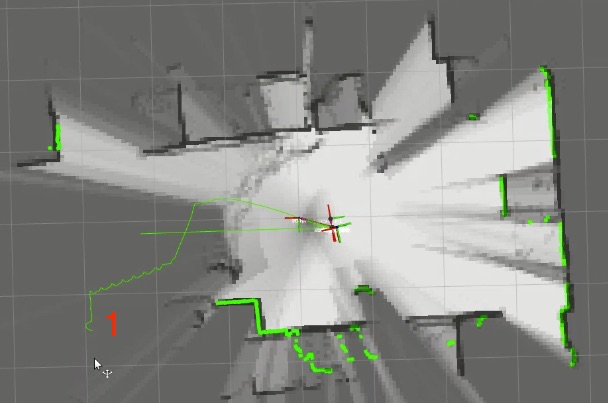
\includegraphics[width=0.97\textwidth]{./imgs/turn_corners/an_frame_1.jpg}
        \caption{Frame 1: Setpoint placed around corner}
        \label{fig:avoid_obs_1}
    \end{subfigure}%
    \begin{subfigure}[b]{0.5\textwidth}
        \centering
        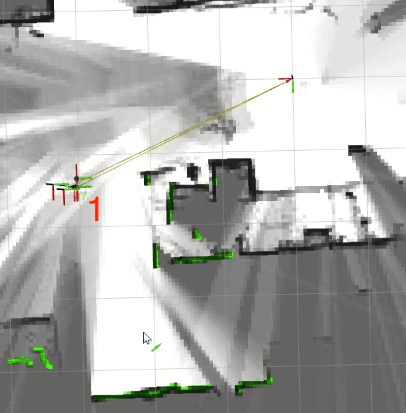
\includegraphics[width=0.97\textwidth]{./imgs/turn_corners/an_frame_2.jpg}
        \caption{Frame 2: Drone reached global setpoint}
        \label{fig:avoid_obs_2}
    \end{subfigure}
    \caption{Experiment showing drone turning corners (1) Global setpoint\label{fig:avoid_obs}}
\end{figure}

Figure \ref{fig:avoid_obs_1} shows a global goal being placed for the drone in an unseen area around the corner.  Note the map has not yet been generated but a goal was able to be placed.  In figure \ref{fig:avoid_obs_1} the drone can be seen to have reached the setpoint.

\subsection{Entering Room}

A final experiment was conducted to test the drones ability to fly through narrow passages.  The format followed the same structure as the above tests.  A global goal placed inside a room and the drone was observed for collisions and ability to reach global goal.

\begin{figure}[H]
    \centering
    \begin{subfigure}[b]{0.5\textwidth}
        \centering
        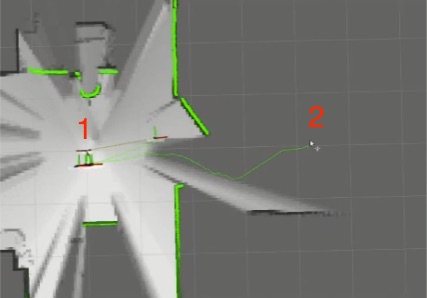
\includegraphics[width=0.97\textwidth]{./imgs/entering_room/an_frame_1.jpg}
        \caption{Frame 1: Global setpoint placed inside room}
        \label{fig:enter_room_1}
    \end{subfigure}%
    \begin{subfigure}[b]{0.5\textwidth}
        \centering
        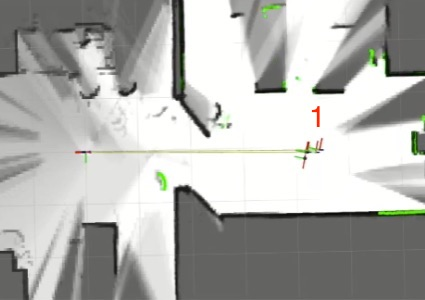
\includegraphics[width=0.97\textwidth]{./imgs/entering_room/an_frame_2.jpg}
        \caption{Frame 2: Drone reached global setpoint}
        \label{fig:enter_room_2}
    \end{subfigure}
    \caption{Experiment showing drone entering room (1) Drone position (2) Global setpoint}
    \label{fig:enter_room}
\end{figure}

Initially a a typical doorway width (0.8m) was used, but was found to be too narrow for the drone to pass through without any collisions.  The cause of this was a result of the drones overshoot.  The gap was increased until the drone was able to pass through safely.  A gap of $1m$ was found to be sufficiently large for the drone to pass through without collisions.
\end{document}